% =============================================
% =============================================
% Document class: Article
\documentclass[ a4paper, twoside, 11pt]{article}
% Packages: LaTeX (Depth-1)
\usepackage[ vlined, linesnumbered, ruled]{algorithm2e}
\usepackage{ amsfonts, amsmath, amssymb, amsthm}
\usepackage[ titletoc, title]{appendix}
\usepackage{ bbm}
\usepackage{ color}
\usepackage{ dsfont}
\usepackage{ enumitem}
\usepackage{ graphicx}
\usepackage{ fancyhdr, float, fullpage}
\usepackage{ hyperref}
\usepackage{ lastpage, latexsym, lipsum}
\usepackage{ mathrsfs, mathtools, multicol}
\usepackage{ parskip}
\usepackage{ setspace, stmaryrd, subcaption}
\usepackage{ tabularx}
\usepackage{ wasysym}
\usepackage[ dvipsnames, table]{ xcolor}
\usepackage{ xfrac}
% Packages: LaTeX (Depth-2)
\usepackage{ epstopdf}

% =============================================
\topmargin 			= -1.6cm
\headheight 		= .90cm
\headsep 			= .80cm
\textheight 		= 24.0cm
\textwidth 			= 15.5cm
\oddsidemargin		= 0.cm
\evensidemargin 	= 0.cm

% =============================================
% =============================================
% Macros: Language
\newcommand{\define}{\triangleq}
\newcommand{\done}{\hfill $\square$}
%\newcommand{\eqCIRC}{\stackrel{\circ}{=}}
%\newcommand{\eqSTAR}{\stackrel{*}{=}}
\renewcommand{\epsilon}{\varepsilon}
\newcommand{\eg}{\textit{e.g.,\;}}
\newcommand{\egc}{\textit{e.g.:\;}}
\newcommand{\Eg}{\textit{E.g.,\;}}
\newcommand{\Egc}{\textit{E.g.:\;}}
\newcommand{\ie}{\textit{i.e.,\;}}
\newcommand{\iec}{\textit{i.e.:\;}}
\newcommand{\Ie}{\textit{I.e.,\;}}
\newcommand{\Iec}{\textit{I.e.:\;}}
\newcommand{\QED}{\hfill $\blacksquare$}
\renewcommand{\tilde}[1]{\widetilde{#1}}
\newcommand{\tsup}[1]{\ensuremath{^{\text{#1}}}}
\newcommand{\tsub}[1]{\ensuremath{_{\text{#1}}}}
\renewcommand{\vec}[1]{{\boldsymbol{#1}}}

% Macros: Optimization & Probability
\DeclareMathOperator*{\argmax}{arg\,max}
\DeclareMathOperator*{\argmin}{arg\,min}
\newcommand{\Exp}{\mathbb{E}}
\newcommand{\Indicate}[1]{ \IndFun \, \{ \, #1 \, \} }
\renewcommand{\Pr}{\mathbb{P}}
\newcommand{\Normal}{\mathcal{N}}
\newcommand{\std}{\text{std}}
\newcommand{\var}{\text{var}}

% Macros: Sets
\newcommand{\Complex}{\mathbb{C}}
\renewcommand{\emptyset}{\varnothing}
\newcommand{\Nat}{\mathbb{N}}
\renewcommand{\Re}{\mathbb{R}}
\newcommand{\ReNN}{{\Re}_{\geq 0}}
\newcommand{\ReSP}{{\Re}_{> 0}}
\renewcommand{\subset}{\subseteq}
\renewcommand{\supset}{\supseteq}
\newcommand{\Z}{\mathbb{Z}}
\newcommand{\ZNN}{{\Z}_{\geq 0}}

% Macros: Spacing & Other Commands
\newcommand{\fullcut}{\vspace{-\baselineskip}}
\newcommand{\fullskip}{\vspace{\baselineskip}}
\newcommand{\halfcut}{\vspace{-0.5\baselineskip}}
\newcommand{\halfskip}{\vspace{0.5\baselineskip}}
\renewcommand{\figurename}{Figura}
\renewcommand{\tablename}{Tabla}

% =============================================
% Sesion de Clase
\newcommand{\sesion}{02}
% Macros para definiciones, teoremas, etc
\newcounter{sesion}
\setcounter{sesion}{\sesion}
\theoremstyle{definition}
\newtheorem{definition}{Definici\'on}[sesion]
\newtheorem{example}[definition]{Ejemplo}
\newtheorem{exercise}[definition]{Ejercicio}
\newtheorem{note}[definition]{Nota}
\newtheorem{problem}[definition]{Problema}
\newtheorem{theorem}[definition]{Teorema}

% =============================================
% =============================================
\newcommand{\HeaderLine}{}
\newcommand{\FooterLine}{P\'agina \thepage ~de \pageref*{LastPage}}

\pagestyle{fancyplain}
\fancyhf{}

\rhead[]{\fancyplain{}{\HeaderLine}}
\lhead[\fancyplain{}{\HeaderLine}]{}
\lfoot[\fancyplain{}{\FooterLine}]{}
\rfoot[]{\fancyplain{}{\FooterLine}}

\renewcommand{\headrulewidth}{0.4pt}
\renewcommand{\footrulewidth}{0.4pt}
\renewcommand{\thefootnote}{\fnsymbol{footnote}}

% =============================================
% =============================================
\begin{document}
\allowdisplaybreaks

\begin{center}
\Large Control Autom\'atico (FIMCP-03905): Examen \sesion \\[1ex]
\small \textbf{A\~no:} 2016-2017 \qquad \textbf{T\'ermino:} II \qquad
\textbf{Instructor:} Luis I. Reyes Castro \qquad \textbf{Paralelo:} 02
\end{center}
\halfskip

\fbox{

\begin{minipage}[b][\height][t]{\textwidth}
\vspace{0.2 cm}

\begin{center}
\textbf{COMPROMISO DE HONOR}
\end{center}
\vspace{0.4 cm}

\scriptsize
{
Yo, \rule{60mm}{.1pt} al firmar este compromiso, reconozco que el presente examen est\'a dise\~nado para ser resuelto de manera individual, que puedo usar un l\'apiz o pluma y una calculadora cient\'ifica, \linebreak que solo puedo comunicarme con la persona responsable de la recepci\'on del examen, y que cualquier instrumento de comunicaci\'on que hubiere tra\'ido debo apagarlo. Tambi\'en estoy conciente que no debo consultar libros, notas, \linebreak ni materiales did\'acticos adicionales a los que el instructor entregue durante el examen o autorice a utilizar. Finalmente, me comprometo a desarrollar y presentar mis respuestas de manera clara y ordenada. \\

Firmo al pie del presente compromiso como constancia de haberlo le\'ido y aceptado. 
\vspace{0.4 cm}

Firma: \rule{60mm}{.1pt} \qquad N\'umero de matr\'icula: \rule{42mm}{.1pt} \hspace{0.5cm} \\[-0.8ex]

}

\end{minipage}

}

\halfskip

\textbf{Instrucciones:} Cada uno de los siguientes cuatro problemas tiene un peso de 10 puntos. 
\halfskip

% =============================================
\begin{problem}
Encuentre la funci\'on de transferencia para cada uno los sistemas mostrados en la figura de abajo. 

\begin{figure}[htb]
\centering
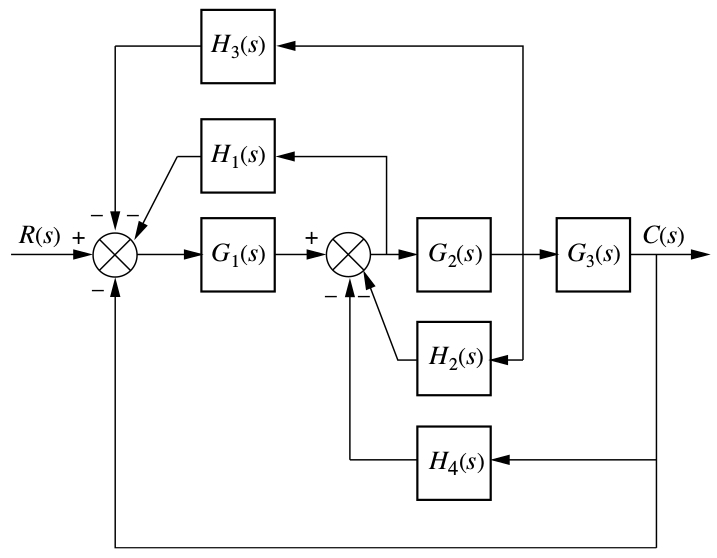
\includegraphics[ width = 0.68\textwidth]{fig_P5-10.jpg} \\[8ex]
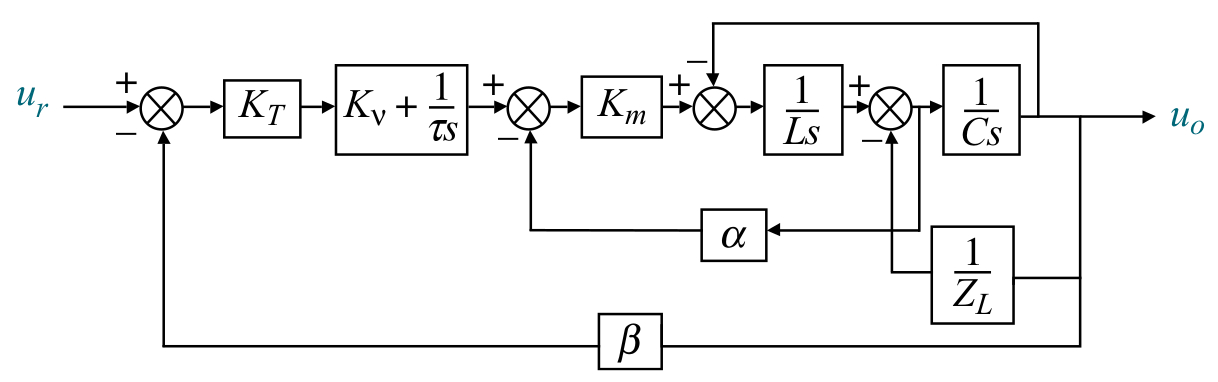
\includegraphics[ width = 0.82\textwidth]{fig_P7-22.jpg}
\end{figure}

\end{problem}
\vspace{\baselineskip}

\newpage

% =============================================
\begin{problem}
Considere el sistema de control de temperatura de un intercambiador de calor que se muestra en la figura de abajo. Suponga que: 
\begin{figure}[htb]
\centering
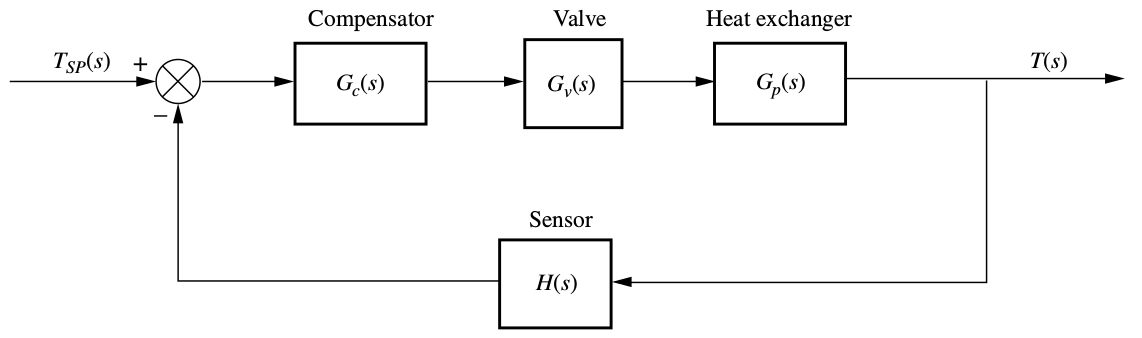
\includegraphics[ width = 0.92\textwidth]{fig_P9-6.jpg}
\end{figure}

\begin{itemize}
\item El intercambiador de calor y el sensor fueron estudiados mediante modelos termo-din\'amicos. En particular: 
\begin{itemize}
\item Para el intercambiador de calor la se\~nal de entrada es la apertura de la v\'alvula $a(t)$ y la se\~nal de salida es la temperatura del intercambiador $T(t)$. Estas se\~nales est\'an relacionadas por la ecuaci\'on diferencial: 
\[
\dot{T}(t) \, = \, -0.02 \, T(t) + 1.4 \, a(t)
\]
\item Para el sensor la se\~nal de entrada es la temperatura del intercambiador de calor $T(t)$ y la salida es la temperatura indicada por el sensor $T_{sensor}(t)$. Estas se\~nales est\'an relacionadas por la ecuaci\'on diferencial: 
\[
\dot{T}_{sensor}(t) \, = \, \left( \frac{1}{12} \right) \, ( \, T(t) - T_{sensor}(t) \, )
\]
\end{itemize}
\item El compensador toma como se\~nal de entrada el error de temperatura $e(t) = T_{SP}(t) - T_{sensor}(t)$ y produce como se\~nal de salida un voltage $v(t)$ que alimenta a la v\'alvula. 
\item La v\'alvula fue estudiada experimentalmente. Dicha v\'alvula toma como se\~nal de entrada el voltage $v(t)$ provisto por el compensador y produce como se\~nal de salida su apertura $a(t)$. Se estim\'o su funci\'on de transferencia como: 
\[
G_v(s) \, = \, \frac{A(s)}{V(s)} \, = \, \frac{0.02}{4s + 1}
\]
\end{itemize}

Con esto en mente: 
\begin{enumerate}[label=\alph*.]
\item Encuentre la funci\'on de transferencia del intercambiador de calor, denotada $G_p(s)$, y del sensor, denotada $H(s)$. Recuerde que: 
\[
G_p(s) \, = \frac{T(s)}{A(s)} \qquad \qquad \qquad H(s) \, = \, \frac{T_{sensor}(s)}{T(s)}
\]
\item Suponiendo que el controlador es proporcional, \ie que $G_c(s) = K$, encuentre el valor de la ganancia $K$ para que el sistema tenga un factor de amortiguamiento $\zeta = 0.7$. 
\item Encuentre el error en estado estable para este sistema cuando la ganancia $K$ toma el valor que usted calcul\'o anteriormente. 
\end{enumerate}

\end{problem}
\vspace{\baselineskip}

% =============================================
\begin{problem}

\begin{figure}[htb]
\centering
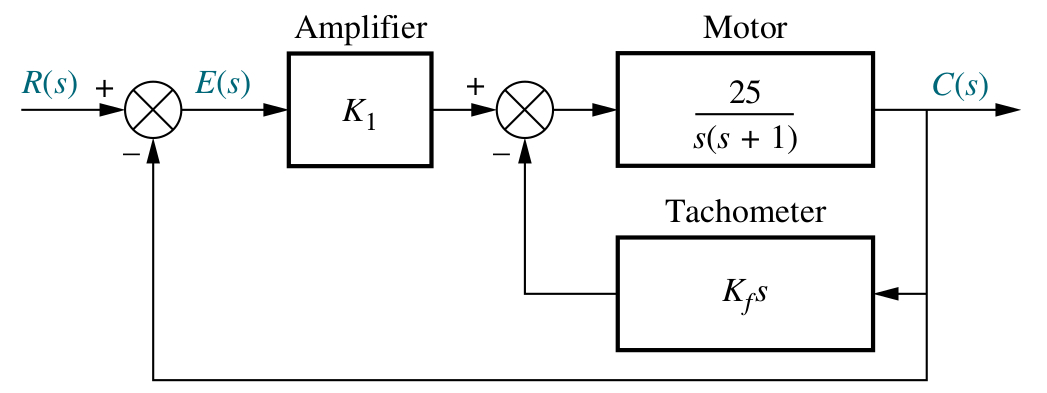
\includegraphics[ width = 0.68\textwidth]{fig_P9-8.jpg}
\end{figure}

Considere el sistema de control de posici\'on angular mostrado en la figura de arriba. Con esto en mente: 
\begin{enumerate}[label=\alph*.]
\item Encuentre valores para las ganancias $K_1$ y $K_f$ de tal manera que las m\'etricas de respuesta en el tiempo del sistema en circuito cerrado sean: 
\begin{itemize}
\item Porcentaje de sobrepaso del 25\%. 
\item Tiempo de asentamiento de 0.2 segundos. 
\end{itemize}
\item Calcule el error en estado estable del sistema en circuito cerrado para una entrada escal\'on $r(t) = u(t)$ y para una entrada rampa $r(t) = t \, u(t)$. 
\end{enumerate}

\end{problem}
\vspace{\baselineskip}

% =============================================
\begin{problem}
Considere el sistema de control de cabeceo de un veh\'iculo a\'ereo no-tripulado mostrado en la figura de abajo. 

\begin{figure}[htb]
\centering
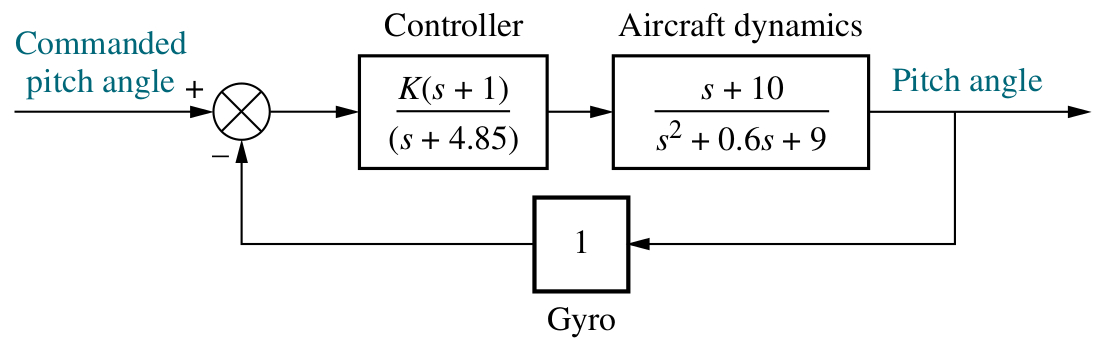
\includegraphics[ width = 0.68\textwidth]{fig_P6-12.jpg}
\end{figure}

Con esto en mente: 
\begin{enumerate}[label=\alph*.]
\item Asumiendo la forma del controlador mostrada en la figura, bosqueje el lugar geom\'etrico de las ra\'ices \emph{(root locus)}. 
\item De acuerdo a su bosquejo anterior, determine la veracidad o falsedad de cada uno de las siguientes proposiciones. 
\begin{itemize}
\item Existe al menos un valor de la ganancia $K$ tal que si $K$ es inferior a ese valor entonces el sistema es estable. 
\item Existe al menos un valor de la ganancia $K$ tal que si $K$ es superior a ese valor entonces el sistema es estable. 
\item Existe al menos un valor de la ganancia $K$ tal que si $K$ es superior a ese valor entonces el sistema es inestable. 
\item El sistema es estable para todos los valores de la ganancia $K$. 
\item Existe un valor de la ganancia $K$ para el cual todos los polos son complejos. 
\item Existe un valor de la ganancia $K$ para el cual todos los polos son reales. 
\end{itemize}
\item Ahora suponga que usted reemplaza el controlador anterior por un controlador PD (\ie proporcional-derivada) cuya funci\'on de transferencia es:
\[
G_{controlador}(s) \, = \, K \, ( \, s + 5.7 \, )
\]
Bosqueje el lugar geom\'etrico de las ra\'ices para esta nueva configuraci\'on del sistema y utilice el bosquejo para responder a las mismas preguntas del literal (b). 
\item Luego suponga que usted reemplaza el controlador anterior por un controlador cuya funci\'on de transferencia es:
\[
G_{controlador}(s) \, = \, \frac{K}{s^2 + 8s + 20}
\]
Bosqueje el lugar geom\'etrico de las ra\'ices para esta nueva configuraci\'on del sistema y utilice el bosquejo para responder a las mismas preguntas del literal (b). 
\item Finalmente, supongamos que el sistema de control que usted est\'a dise\~nando es para un avi\'on de juguete. El juguete debe ser econ\'omico, \ie barato, por lo que su jefe le orden\'o escoger el controlador m\'as sencillo de entre los tres controladores considerados, d\'onde ``m\'as sencillo'' se define en t\'erminos del n\'umero de polos y ceros del controlador. Con esto en mente, cu\'al controlador escoger\'ia para el juguete que est\'a dise\~nando? 

\end{enumerate}

\end{problem}
\vspace{\baselineskip}

%% =============================================
%\begin{problem} Considere el siguiente modelo de las din\'amicas longitudinales de un caza-bombardero F4-E Phantom representado como modelo de espacio de estados. En este modelo, los estados son la aceleraci\'on normal, denotada $a_n(t)$, la velocidad del \'angulo de inclinaci\'on de la nariz, denotada $q(t)$, y el \'angulo del elevador horizontal, denotado $\delta_e(t)$. 
%\begin{align*}
%& \frac{d}{dt}
%\left[ \begin{array}{c}
%a_n(t) \\ q(t) \\ \delta_e(t)
%\end{array} \right] \, = \, 
%\left[ \begin{array}{ccc}
%-1.70 & 50.7 & 263.4 \\
%0.22 & -1.42 & -32 \\
%0 & 0 & -14
%\end{array} \right] 
%\left[ \begin{array}{c}
%a_n(t) \\ q(t) \\ \delta_e(t)
%\end{array} \right]
%+ \left[ \begin{array}{c}
%-272.1 \\ 0 \\ 14
%\end{array} \right] \delta_{com}(t)
%\end{align*}
%
%Con esto en mente, encuentre: 
%\begin{itemize}
%\item La matrices $C$ y $D$ para el caso cuando la salida es la aceleraci\'on normal $a_n(t)$. 
%\item La funci\'on de transferencia: 
%\[
%G(s) \, \define \, \frac{A_n(s)}{\Delta_{com}(s)}
%\]
%\end{itemize}
%
%\end{problem}
%\vspace{\baselineskip}

\end{document}
